% ============================================================
% f2015tjl_q05_circle.tex —— 2015 天津卷（理科）第 5 题 圆与割线
% ------------------------------------------------------------
% 坐标口径：图内画布 pt，原点 = 源页基准点，x 右正、y 上正。
%   来源：.work/phase3-b11/figure-inventory.md（真实页 pt，原点左上、y 向下）
%   换算：X_tikz = x_page − 169.40 ；  Y_tikz = 773.78 − y_page
% 线宽：圆 0.398 pt；弦 AB 0.398 pt（图形本体档，清单未单独标注，取本体档）；
%       两割线 CE / CD **0.42 pt**（清单 §2.3 实测值，源图自身与他线不同档，照源保留）。
% 照源复刻（清单 §7 存疑）：
%   S-3 圆心实心点为**字形** U+2022（\textbullet），非矢量填充；与「O」并置为「•O」，
%       字形落于文字基线，其墨迹中心较几何圆心 (53.895,53.890) 有约 3.6 pt 垂直偏置。
%   S-4 两割线在弦高 y=736.90 处与三等分点 M/N 有 1.65 / 0.49 pt 微差（源图未精确
%       满足题设交点约束）——**照源复刻，不「修正」**。
% 要素：3 描边 path（圆 / 弦 / 两割线合一）+ 8 文字标签（清单 §2.6）。
% ============================================================
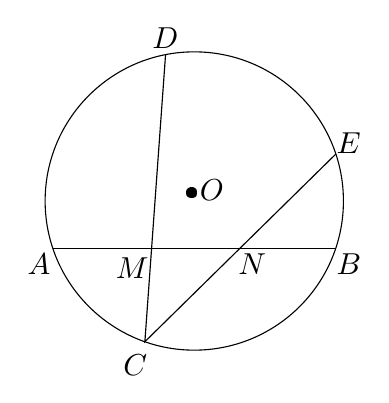
\begin{tikzpicture}[
  x=1pt,y=1pt,                             % 画布单位 = 1 pt（本文件坐标一律为 pt）
  every node/.style={font=\fontsize{10.5pt}{12.6pt}\selectfont,inner sep=0pt},
  body/.style={line width=0.398pt},
  sec/.style={line width=0.420pt},
]

  % ---------- 圆（圆心 (223.295,719.890)，r = 53.895）----------
  \draw[body] (53.895,53.890) circle [radius=53.895pt];

  % ---------- 弦 AB（水平全长弦，(172.10,736.90)→(274.50,736.90)，长 102.40）----------
  \draw[body] (2.70,36.88) -- (105.10,36.88);

  % ---------- 两割线（源图为 1 个 path 的 2 个子段，共点 C）----------
  % CE：E(274.49,702.88) → C(205.44,770.75)
  % CD：C(205.44,770.75) → D(212.92,666.99)
  \draw[sec] (105.09,70.90) -- (36.04,3.03) -- (43.52,106.79);

  % ---------- 标签（清单 §2.5 实测字形中心）----------
  \node at (-2.20,30.98)  {$A$};
  \node at (109.80,30.98) {$B$};
  \node at (32.60,-5.32)  {$C$};
  \node at (43.40,112.78) {$D$};
  \node at (109.70,74.88) {$E$};
  \node at (31.50,29.58)  {$M$};
  \node at (74.80,30.98)  {$N$};

  % ---------- 圆心「•O」：U+2022 字形与 O 并置（S-3 照源）----------
  \node at (57.495,57.86) {\textbullet $O$};

\end{tikzpicture}
